\documentclass[11pt]{amsart}
\usepackage{amsmath}
\usepackage{geometry}                % See geometry.pdf to learn the layout options. There are lots.
\geometry{letterpaper}                   % ... or a4paper or a5paper or ... 
%\geometry{landscape}                % Activate for for rotated page geometry
%\usepackage[parfill]{parskip}    % Activate to begin paragraphs with an empty line rather than an indent
\usepackage{graphicx}
\usepackage{caption}
\usepackage{subcaption}
\usepackage{amssymb}
\usepackage{epstopdf}
\usepackage[]{algorithm2e}
\usepackage{tikz}
\usetikzlibrary{positioning}
\usepackage{intcalc}
\usepackage{blkarray}


\newcommand{\vek}[1]{\mathbf{#1}}
\DeclareMathOperator*{\argmax}{argmax}

\graphicspath{{Figures/}}

\title{Comp 652: Assignment 3}
\author{Carlos G. Oliver (260425853)}
\date{\today}                                           % Activate to display a given date or no date

\begin{document}
\maketitle

\section{Q1: PCA}

\begin{figure}[h]
\centering
\begin{subfigure}{0.5\textwidth}
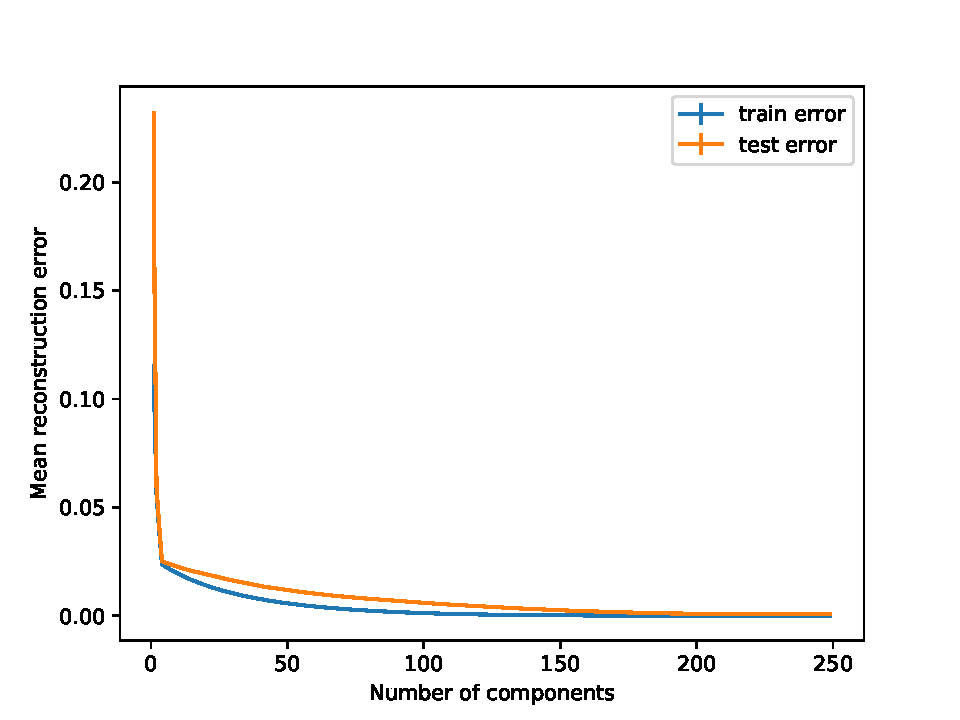
\includegraphics[width=\textwidth]{reconstruction.pdf}
\caption{}
\label{subfig:rfam_count}
\end{subfigure}
~
\begin{subfigure}{0.46\textwidth}
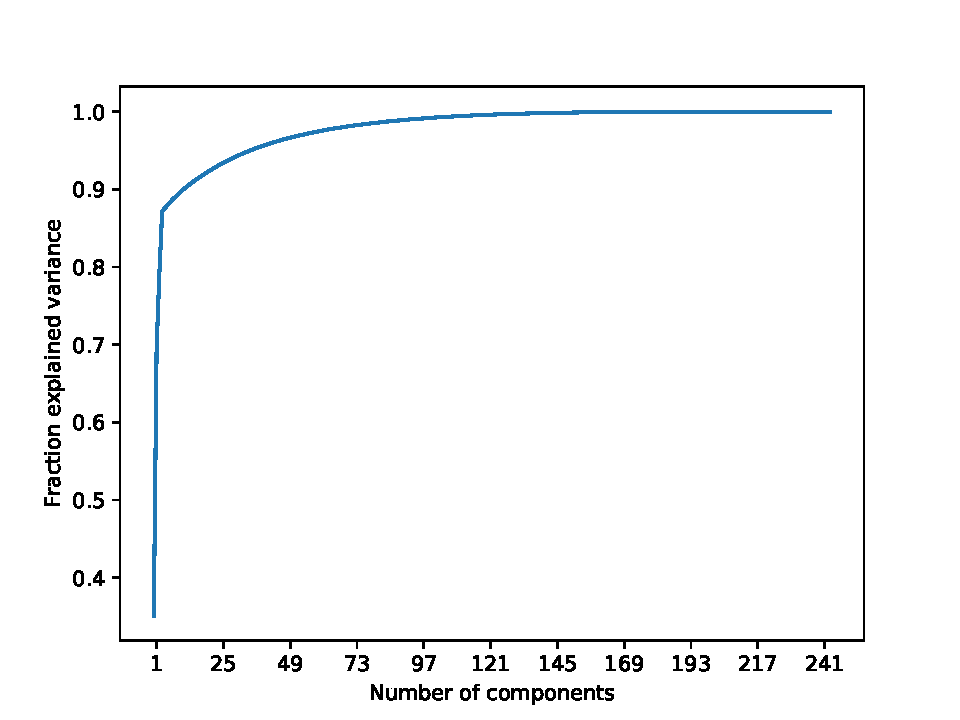
\includegraphics[width=\textwidth]{var.pdf}
\caption{}
\label{subfig:rfam_stats}
\end{subfigure}

\caption{}
\label{fig:rfam}
\end{figure}

\section{Q2: Spectral methods for weighted automata}
\subsection{(a)}

We use a property of Hankel matrices which is: if $\text{rank}(H_f) = n \Rightarrow$ there exists a weighted finite automaton $\mathcal{A}$  with $n$ states such that $g = g_{\mathcal{A}}$ for some function $g : \Sigma^{*} \rightarrow \mathbb{R}$ where $\Sigma^{*}$ is the set of all strings that can be generated from alphabet $\Sigma$. In this example, the function $g$ counts the number of $1$s in a string generated from $\Sigma = \{0, 1\}$ the Hankel matrix $H_g$ would take the form: 


 
\[
H_g = \begin{blockarray}{cccccc}
\def\ra{\color{red}\ba}
 & \lambda & 0 & 1 & 11 & \hdots \\
\begin{block}{c[ccccc]}
  \lambda & 0 & 0 & 1 & 2 & \hdots \\
  0 & 0 & 0 & 1 & 2 &  \\
  1 & 1 & 1 & 2 & 3 &  \\
  11 & 2 & 2 & 3 & 4 &  \\
  111 & 3 & 3 & 4 & 5 &  \\
  110 & 2 & 2 & 3 & 4 &  \\
  \vdots & \vdots &  &  &  & \ddots \\
\end{block}
\end{blockarray}
\label{mat:h_1}
 \]

The above matrix is arranged so all possible strings composed only of $1$s, $Q = \{1\}^N \quad \forall N \in \mathbb{Z^+}$ precede all other strings ($\Sigma^{*} - Q$) with the exception of $\{0\}^1$ and $\lambda$. If we order prefixes and suffixes in S in increasing $N$ we can easily see that any row $m$ in this sub block $H^{1}_g$ of $H_g$ is a linear combination in the form $H^{1}_g(m, \cdot) = 2H^{1}_g(m, \cdot) - H^{1}_g(m-1, \cdot)$. The remaining entries in $H_g$ are formed by prefixes and suffixes containing $0$s which do not contribute to the evaluation of $g$ and therefore can also be obtained from rows or columns in $H^{1}$. Therefore the rank of $H_g$ is 2 where only the $\lambda$ or $\{0\}^1$ and the $\{1\}^1$ contribute to the row rank. The same can be shown for the column rank.

\subsection{(b)}

If $f$ is a probability distribution over $\Sigma^*$ then we have $\sum_{s \in \Sigma^*} f(s) = 1$ gives a probability for every string in $\Sigma^*$. Then $f_{sub}(w)$ is the probability that the string $w$ occurs in any word generated by $\Sigma^*$ since $u$ and $v$ represent all possible prefixes and suffixes to the word $w$.

\subsection{(c)}

Let $ \Sigma_{w \in \Sigma^*} A_w \equiv S$.

\begin{equation}
\begin{aligned}
S = (I - A_0 - A_1)^{-1} = (I - A_0 - A_1) S          &= I \\
				       (I - A_0 - A_1)SS^{-1} &= S^{-1}	\\
				       (I - A_0 - A_1)^{-1} 	&= S
\end{aligned}
\end{equation}

Now we use this identity to compute the sum of the function $f$ over all words as $ \Sigma_{w \in \Sigma^*} f(w)$. We can express the function over a string as

\begin{equation}
\begin{aligned}
f(w) = \alpha_0^T Aw \alpha_{\infty}
\end{aligned}
\end{equation}

So for all the words we have
\begin{equation}
\begin{aligned}
\sum_{w \in \Sigma^*} f(w) &= \sum_{w \in \Sigma^*} \alpha_0^T A_w \alpha_{\infty} \\
					 &= \alpha_0^T \bigg( \sum_{w \in \Sigma^*}  A_w  \bigg) \alpha_{\infty} \\
					 &= \alpha_0^T (I - A_0 - A_1)^{-1} \alpha_{\infty}
\end{aligned}
\end{equation}
We can use this property to compute $f_{subsrting}(w)$ using an automaton by recognizing that the contribution of transition matrices from $u$ and $v$ to the sum can be reduced to the same identity as above as they sum over all of $\Sigma^*$.

\begin{equation}
\begin{aligned}
f_{substring} (w)  &= \sum_{u \in \Sigma^*, v \in \Sigma^*} f(uwv) \\
			 &=  \sum_{u \in \Sigma^*, v \in \Sigma^*} \alpha_0^T A_u A_w A_v \alpha_{\infty} \\
			 &=   \alpha_0^T (I - A_0 - A_1)^{-1}  A_w (I - A_0 - A_1)^{-1}  \alpha_{\infty}
\end{aligned}
\end{equation}

\subsection{(d)}

Because the word $uwv$ is in $\Sigma^*$ and the training sample $S$ is drawn from $f$ also over $\Sigma^*$, having an automaton that represents this function would also give us a way to learn the function $f_{substring}$. From $S$ we can construct the empirical Hankel matrix $\hat{H}_{f_{substring}}$ and recover the relevant sub-blocks. We can then perform SVD on $H$ and solve for the necessary transition weights $A_w$ and initial/final vecctors $\alpha_0$, $\alpha_{\infty}$ from which we can produce the weighted automaton $\hat{A}$. In order to recover an estimate of $f$ we would have to sample from the automaton over all $w \in \Sigma^*$ as this would compute the probability distribution over all words in $\Sigma^*$. 


\section{Q3: Method of moments and multiview model}

\begin{figure}[h]
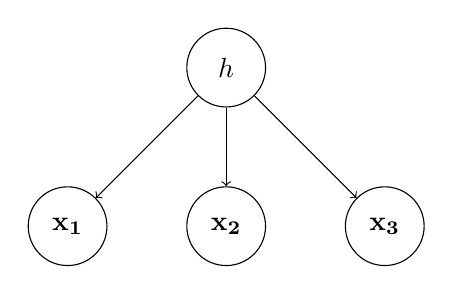
\begin{tikzpicture}[
  vertex/.style={draw,circle,minimum size=1cm},
  every node/.style={vertex}
  ]
	 \node (h) at (0,0) {$h$};
	  \node [below = of h] (x2) {$\vek{x_2}$};
	 \node [left = of x2]  (x1) {$\vek{x_1}$};	
	 \node [right = of x2] (x3) {$\vek{x_3}$};
	 
	 \draw [->] (h) edge (x1) (h) edge (x2) (h) edge (x3);
\end{tikzpicture}
\caption{Graphical representation of conditional independence relation between random variables $\vek{x_1, x_2, x_3}$ and $h$.}
\label{fig:graph}
\end{figure}

Since the $\vek{x_t}$ are conditionally independent given $h$ we can decompose the conditional expectation of the cross moments.

\begin{equation}
\begin{aligned}
\mathbb{E}[\vek{x_1} \otimes \vek{x_2} \vert h=j] &= \mathbb{E}[\vek{x_1} \vert h=j] \otimes \mathbb{E}[\vek{x_2} \vert h=j] && \text{by conditional independence} \\
								           &= \mu_{t=1, j} \otimes \mu_{t=2, j}  \in \mathbb{R}^{d_1 \times d_2}&& \text{by question statement}\\
								           &= \sum_{i=1}^k w_i \mu_{1,i} \otimes \mu_{2, i}
\end{aligned}
\end{equation}

\begin{equation}
\begin{aligned}
\mathbb{E}[\vek{x_1} \otimes \vek{x_2} \otimes \vek{x_3} \vert h=j] &= \sum_{i=1}^k w_i \mu_{1,i} \otimes \mu_{2, i} \otimes \mu_{3, i} \in \mathbb{R}^{d_1 \times d_2 \times d_3}
\end{aligned}
\end{equation}

Because the tensor products of the $\vek{x_t}$ give rise to non-symmetric tensors, we cannot apply the standard tensor method of moments as eigenvalue decomposition requires symmetric matrices ~\cite{anandkumar2014tensor}. Other techniques can be employed but are beyond the scope of this question.

\section{Q4: Coupled Hidden Markov Models}

\subsection{(a)}

Parametrization of CHMM:

\begin{itemize}

\item Initial probabilities:
\begin{equation}
\begin{aligned}
P(s_0 = s) && \forall s \in S \\
P(u_0 = u) && \forall u \in U
\end{aligned}
\end{equation}

\item Transition Probabilities
\begin{equation}
\begin{aligned}
P(s_{t+1} = s' \vert s_{t-1} = s, u_{t-1} = u) && \forall s', s, u \in S \cup U\\
P(u_{t+1} = u' \vert u_{t-1} = u, s_{t-1} = s) && \forall u', u, s \in S \cup U
\end{aligned}
\end{equation}

\item Emission Probabilities
\begin{equation}
\begin{aligned}
P(y_t = y \vert s_t = s) && \forall s \in S, y \in Y \\
P(z_t = y \vert u_t = u) && \forall u \in U, z \in Z
\end{aligned}
\end{equation}

\end{itemize}

\subsection{(b)}

We want to compute $P((y_0, z_0), (y_1, z_1), ...(y_T, z_T))$. We can obtain this probability by marginalizing over the states in the joint over the full model. 

\begin{equation}
\begin{aligned}
&P((y_0, z_0), \ldots, (y_T, z_T)) \\
 &= \sum_{s_0, \ldots, s_T, u_0, \ldots u_T} P((y_0, z_0),  \ldots (y_T, z_T), s_0, \ldots, s_T, u_0, \ldots, u_T) \\
								 &= \sum_{s_0, \ldots, s_T, u_0, \ldots u_T} P(s_0) P(u_0) \prod_{t=1}^{T} P(s_t \vert s_{t-1}, u_{t-1}) \prod_{t=1}^{T} P(u_t \vert s_{t-1}, u_{t-1}) \prod_{t=0}^{T} P(y_t \vert s_T) \prod_{t=0}^{T} P(z_t \vert u_t) \\
								 &= \sum_{s_T} P(y_T \vert s_T) \sum_{u_T} P(z_T \vert u_T) \sum_{s_0, \ldots, s_{T-1}, u_0, \ldots u_{T-1}} P(s_T \vert s_{T-1}) P(u_T \vert u_{t-1}) P(s_0) P(u_0)\\
								 & \qquad  \prod_{t=1}^{T-1} P(s_t \vert s_{t-1}, u_{t-1}) \prod_{t=1}^{T-1} P(u_t \vert s_{t-1}, u_{t-1})
\end{aligned}
\label{eq:hmm1}
\end{equation}

We obtain the second step simply by factoring the graph into its independent components according to the graphical model. By rearranging terms we see that the full joint distribution can be written as a product of the distribution at the final time $T$ and the joint over all times $T-1$ which suggests a dynamic programming algorithm which we can write in the following form:

\begin{equation}
\begin{aligned}
P((y_0, z_0),...(y_T, z_T)) &= \sum_{s_T, u_T} P((y_0, z_0), (y_1, z_1), ...(y_T, z_T), u_T, s_T) \\
					&= \sum_{s_T, u_T} P(z_T \vert u_T) P(y_T \vert s_T) \sum_{S_{T-1}} P(s_T \vert s_{T-1}) P(u_T \vert u_{T-1}) P((y_0, z_0), ...(y_T, z_T), s_{T-1}, u_{T-1})
\end{aligned}
\end{equation}

We define a matrix $A_{t}(s, u)$ of dimensions $\vert S \vert$ and $\vert U \vert$ that will store the probability of the observation sequence until time $t$ and of state $s_t$ and $u_t$. In the uncoupled version of HMM we have a vector instead of a matrix. The entries of this matrix have the following form:

\begin{equation}
A_{t}(s,u) = P((y_0, z_0),...(y_t, z_t), s_t=s, u_t=u)
\end{equation}

At $t=0$ we have our base case which is a function of the initial probabilities $s_0$ and $u_0$:

\begin{equation}
A_{0}(s,u) = P(y_0, z_0, u_0=u, s_0=s) = P(s_0 =s )p(u_0 = u) P(y_0 \vert s_0 = s)P(z_0 \vert s_0=s) \qquad \forall s,u \in S, U
\end{equation}

For all subsequent time steps $t=1,... t=T$ we can use the recursive expression derived in (\ref{eq:hmm1}):

\begin{equation}
\begin{aligned}
A_t(s,u) = P(y_t \vert s_t) P(z_t \vert u_t) \sum_{s_{t-1}, u_{t-1}} P(s_t \vert s_{t-1}, u_{t-1}) P(u_t \vert s_{t-1}, u_{t-1}) A_{t-1}(s, t)
\end{aligned}
\end{equation}

Rewriting this in more compact form:

\begin{equation}
P(y_0, z_0),...(y_t, z_t)) = \sum_{s_T, u_T} A_{T}(s,u)
\end{equation}

\subsection{(c)}

This task can be accomplished with a modified version of the Viterbi algorithm which is a dynamic programming technique.

We wish to compute the set of hidden states with the maximum probability given the observed sequence:

\begin{equation}
\argmax_{s_0 u_0, s_1 u_1, ..., s_T u_T} P(s_0 u_0, s_1 u_1, ..., s_T u_T \vert (y_0, z_0),...(y_t, z_t))
\end{equation}

Using simple rules of probability we can rewrite the conditional probability:

\begin{equation}
\argmax_{s_0 u_0, s_1 u_1, ..., s_T u_T} \frac{P(s_0 u_0, s_1 u_1, ..., s_T u_T, (y_0, z_0),...(y_t, z_t))}{P((y_0, z_0),...(y_t, z_t))}
\end{equation}

We note that the denominator is just the probability of the observation sequence and does not depend on the hidden states so we can omit it from further calculations. 

Now we can adapt the Viterbi algorithm (as described on Wikipedia) as follows:

To simplify notation we let:

\begin{equation}
\begin{aligned}
P(u_t=u' \vert u_{t-1} = u) &\equiv \mathbb{U}_{u, u'}\\
P(s_t=s' \vert s_{t-1} = s) &\equiv \mathbb{S}_{s, s'}
\end{aligned}
\end{equation}

Now we consider the observed sequence $y_0z_0, y_1z_1, ..., y_t, z_t$. Let the probability of the {\it most likely} state sequence $s_0u_0, s_1u_1, ... s_iu_j$ ending at states $i \in S$ and $j \in U$ be stored in the 3D matrix $V$ where

\begin{equation}
\begin{aligned}
V_{0, i, j} = P(y_0 \vert i) P(z_0 \vert j) P(s_0) P(u_0)
\end{aligned}
\end{equation}

Is the sequence at $t=0$ so we just have the emission probabilities multiplied by the initial state probabilities. For subsequent time steps we have the same as above, instead now we include transition probability factors instead of initial state probabilities, as well as the probability of the sequence of states which led to time $t$ which is just $V_{t-1, s, u}$:

\begin{equation}
V_{t, i, j} = \argmax_{s \in S, u \in U} P(y_t \vert i) P(z_t \vert j) \mathbb{S}_{s, i} \mathbb{U}_{u, j} V_{t-1, s, u}
\end{equation}

This will result in a dynamic programming table storing the probability of all possible paths through the CHMM. Instead of a 2D table as in the standard Viterbi algorithm we will have a 3D table of dimensions $|T| \times |S| \times |U|$. To retrieve the most likely sequence of hidden states, we store back pointers at every $V_t$ that lead to the state that maximized $V_{t-1}$. 

\subsection{(d)}

If chains are coupled every $k$ time steps, then for time steps that are multiples of $k$ we have the same form as the CHMM and for those that are not multiples of $k$ we have two independent chains. This would allow us to decompose the probabilities for time steps in parts (b) and (c) into those that are multiples of $k$ i.e. $\{ t \in \pi_{k} \qquad \text{if} \qquad t \mod k = 0 \}$  and thus remain as before, and those that are not multiples of $k$, i.e. $t \notin \pi_k$ and there is no dependence between chains.



\section{Notes}
Collaboration with Navin Mordani and Jeremy Georges-Filtreau.

\bibliographystyle{plain}
\bibliography{a3_cgo}

\end{document}  